\documentclass[table]{beamer}
%[]中可以使用draft、handout、screen、transparency、trancompress、compress等参数

%指定beamer的模式与主题
\mode<presentation>
{
  \usetheme{Madrid}
%\usetheme{Boadilla}
%\usecolortheme{default}
%\usecolortheme{orchid}
%\usecolortheme{whale}
%\usefonttheme{professionalfonts}
}

%\usetheme{Madrid}
%这里还可以选择别的主题:Bergen, Boadilla, Madrid, AnnArbor, CambridgeUS, Pittsburgh, Rochester, Warsaw, ...
%有导航栏的Antibes, JuanLesPins, Montpellier, ...
%有内容的Berkeley, PaloAlto, Goettingen, Marburg, Hannover, ...
%有最小导航栏的Berlin, Ilmenau, Dresden, Darmstadt, Frankfurt, Singapore, Szeged, ...
%有章和节表单的Copenhagen, Luebeck, Malmoe, Warsaw, ...

%\usecolortheme{default}
%设置内部颜色主题(这些主题一般改变block里的颜色);这个主题一般选择动物来命名
%这里还可以选择别的颜色主题,如默认的和有特别目的的颜色主题default,structure,sidebartab,全颜色主题albatross,beetle,crane,dove,fly,seagull,wolverine,beaver

%\usecolortheme{orchid}
%设置外部颜色主题(这些主题一般改变title里的颜色);这个主题一般选择植物来命名
%这里还可以选择别的颜色主题,如默认的和有特别目的的颜色主题lily,orchid,rose

%\usecolortheme{whale}
%设置字体主题;这个主题一般选择海洋动物来命名
%这里还可以选择别的颜色主题,如默认的和有特别目的的颜色主题whale,seahorse,dolphin

%\usefonttheme{professionalfonts}
%类似的还可以定义structurebold,structuresmallcapsserif,professionalfonts

% 控制 beamer 的风格,可以根据自己的爱好修改
%\usepackage{beamerthemesplit} %使用 split 风格
%\usepackage{beamerthemeshadow} %使用 shadow 风格
%\usepackage[width=2cm,dark,tab]{beamerthemesidebar}

%插入音标
%\usepackage{tipa}
%\AtBeginDocument{
  %\renewcommand\textipa{\fontencoding{T3}\selectfont}
%}
%\AtBeginDocument{
  %\renewcommand\textipa[2][r]{{\fontfamily{cm#1}\tipaencoding #2}}
%}
%\renewenvironment{IPA}[1][r]
 %{\fontfamily{cm#1}\tipaencoding}
 %{}

% 设定英文字体
%\usepackage{fontspec}
% Fix bugs for fontspec in TeXLive2015
\ifdefined\suppressfontnotfounderror
  \expandafter\let\csname xetex_suppressfontnotfounderror:D\endcsname
    \suppressfontnotfounderror
\else
  \expandafter\let\csname xetex_suppressfontnotfounderror:D\endcsname
    \luatexsuppressfontnotfounderror
\fi
\usepackage[no-math]{fontspec}
\setmainfont{Times New Roman}
\setsansfont{Arial}
\setmonofont{Courier New}

% 设定中文字体
\usepackage[BoldFont,SlantFont,CJKchecksingle,CJKnumber]{xeCJK}
%\setCJKmainfont[BoldFont={Adobe Heiti Std},ItalicFont={Adobe Kaiti Std}]{Adobe Song Std}
\setCJKmainfont[BoldFont={Adobe Heiti Std},ItalicFont={Adobe Kaiti Std}]{WenQuanYi Micro Hei}
\setCJKsansfont{Adobe Heiti Std}
\setCJKmonofont{Adobe Fangsong Std}
\punctstyle{hangmobanjiao}

\defaultfontfeatures{Mapping=tex-text}
\usepackage{xunicode}
\usepackage{xltxtra}

\XeTeXlinebreaklocale "zh"
\XeTeXlinebreakskip = 0pt plus 1pt minus 0.1pt

\usepackage{setspace}
\usepackage{colortbl,xcolor}
\usepackage{hyperref}
%\hypersetup{xetex,bookmarksnumbered=true,bookmarksopen=true,pdfborder=1,breaklinks,colorlinks,linkcolor=blue,filecolor=black,urlcolor=cyan,citecolor=green}
\hypersetup{xetex,bookmarksnumbered=true,bookmarksopen=true,pdfborder=1,breaklinks,colorlinks,linkcolor=cyan,filecolor=black,urlcolor=blue,citecolor=green}

% 插入图片
\usepackage{graphicx}
\graphicspath{{figures/}}
% 图文混排
%\usepackage{picins}
\usepackage{floatflt}

% 可能用到的包
\usepackage{amsmath,amssymb}
%插入多媒体
%\usepackage{media9}
%\usepackage{movie15}
\usepackage{multimedia}
\usepackage{multicol}
\usepackage{multirow}

% 定义一些自选的模板,包括背景、图标、导航条和页脚等,修改要慎重
% 设置背景渐变由10%的红变成10%的结构颜色
%\beamertemplateshadingbackground{red!10}{structure!10}
%\beamertemplatesolidbackgroundcolor{white!90!blue}
% 使所有隐藏的文本完全透明、动态,而且动态的范围很小
\beamertemplatetransparentcovereddynamic
% 使itemize环境中变成小球,这是一种视觉效果
\beamertemplateballitem
% 为所有已编号的部分设置一个章节目录,并且编号显示成小球
\beamertemplatenumberedballsectiontoc
% 将每一页的要素的要素名设成加粗字体
\beamertemplateboldpartpage

% item逐步显示时,使已经出现的item、正在显示的item、将要出现的item呈现不同颜色
\def\hilite<#1>{
 \temporal<#1>{\color{gray}}{\color{blue}}
    {\color{blue!25}}
}

\renewcommand{\today}{\number\year 年 \number\month 月 \number\day 日}

%五角星
\usepackage{MnSymbol}

%去除图表标题中的figure等
\usepackage{caption}
\captionsetup{labelformat=empty,labelsep=none}

\usepackage{tabu}
\usepackage{multirow}
%表格自动换行
\usepackage{tabularx} 

% 千分号
%\usepackage{textcomp}

%罗马数字
\makeatletter
\newcommand{\rmnum}[1]{\romannumeral #1}
\newcommand{\Rmnum}[1]{\expandafter\@slowromancap\romannumeral #1@}
\makeatother

%分栏
\usepackage{multicol}

%\usepackage{enumitem}
%\usepackage{enumerate}

%键盘
\usepackage{keystroke}

%插入源代码
\usepackage{listings}
\lstset{
  language=perl,                  % 程序语言名称:TeX, Perl, R, sh, bash, Awk
  basicstyle=\normalsize\tt,      %\tt指monospace字体族,程序源代码使用此族字体表示更加美观
  numbers=left,                   % 行号位置(左侧)
  numberstyle=\small,             % 行号字体的字号
  stepnumber=1,                   % 行号的显示步长
  numbersep=5pt,                  % 行号与代码间距
  backgroundcolor=\color{white},  % 背景色;需要 \usepackage{color}
  showspaces=false,               % 不显示空格
  showstringspaces=false,         % 不显示代码字符串中的空格标记
  showtabs=false,                 % 不显示 TAB
  tabsize=4, 
  frame=shadowbox,                % 把代码用带有阴影的框圈起来
  captionpos=b,                   % 标题位置
  breaklines=true,                % 对过长的代码自动断行
  breakatwhitespace=false,        % 断行只在空格处
  extendedchars=false,            % 解决代码跨页时,章节标题,页眉等汉字不显示的问题
  %escapeinside={\%*}{*},         % 跳脱字符,添加注释,暂时离开 listings 
  %escapeinside=``,
  commentstyle=\color{red!50!green!50!blue!50}\tt,  %浅灰色的注释
  rulesepcolor=\color{red!20!green!20!blue!20},     %代码块边框为淡青色
  keywordstyle=\color{blue!70}\bfseries\tt,         %代码关键字的颜色为蓝色,粗体
  identifierstyle=\tt,
  stringstyle=\tt,                % 代码字符串的特殊格式
  keepspaces=true,
  breakindent=1em,
  %breakindent=22pt,
  %breakindent=4em,
  breakautoindent=true,
  flexiblecolumns=true,
  aboveskip=1em,                  %代码块边框
  xleftmargin=2em,
  xrightmargin=2em
}

%\setbeamercolor{alerted text}{fg=magenta}
\setbeamercolor{bgcolor}{fg=yellow,bg=cyan}
%\setbeamercolor{itemize/enumerate body}{fg=green}

\begin{document}

%\includeonlyframes{current}

\logo{
\includegraphics[height=0.08\textwidth]{tijmu.png}}

% 在每个Section前都会加入的Frame
\AtBeginSection[]
{
  \begin{frame}<beamer>
    %\frametitle{Outline}
    \frametitle{教学提纲}
    \setcounter{tocdepth}{3}
    \begin{multicols}{2}
      \tableofcontents[currentsection,currentsubsection]
      %\tableofcontents[currentsection]
    \end{multicols}
  \end{frame}
}
% 在每个Subsection前都会加入的Frame
\AtBeginSubsection[]
{
  \begin{frame}<beamer>
%%\begin{frame}<handout:0>
%% handout:0 表示只在手稿中出现
    \frametitle{教学提纲}
    \setcounter{tocdepth}{3}
    \begin{multicols}{2}
    \tableofcontents[currentsection,currentsubsection]
    \end{multicols}
%% 显示在目录中加亮的当前章节
  \end{frame}
}

% 为当前幻灯片设置背景
%{
%\usebackgroundtemplate{
%\vbox to \paperheight{\vfil\hbox to
%\paperwidth{\hfil
\includegraphics[width=2in]{tijmu_charcoal.png}\hfil}\vfil}
%}
\begin{frame}[plain]
  \begin{center}
    {\Huge 分子生物计算\\}
    {\huge \textit{(Perl语言编程)}\\}
    \vspace{1cm}
    {\LARGE 天津医科大学\\}
    %\vspace{0.2cm}
    {\LARGE 生物医学工程与技术学院\\}
    \vspace{1cm}
    {\large 2016-2017学年上学期(秋)\\ 2014级生信班}
  \end{center}
\end{frame}
%}



\title[子程序和Bugs]{第六章\quad 子程序和Bugs}
\author[Yixf]{伊现富(Yi Xianfu)}
\institute[TIJMU]{天津医科大学(TIJMU)\\ 生物医学工程与技术学院}
\date{2016年11月}

\begin{frame}
  \titlepage
\end{frame}

\begin{frame}[plain,label=current]
  \frametitle{教学提纲}
  \setcounter{tocdepth}{3}
  \begin{multicols}{2}
    \tableofcontents
  \end{multicols}
\end{frame}



\section{引言}
\begin{frame}
  \frametitle{子程序和Bugs | 引言}
  \begin{block}{子程序(subroutine)}
    \begin{itemize}
      \item 对程序进行结构化组织的一个重要方法。
      \item 类似于shell编程语言中的函数
    \end{itemize}
  \end{block}
  \pause
  \begin{block}{Perl调试器(debugger)}
    用“慢镜头”的形式来检查一个程序的行为,帮助找到bugs。
  \end{block}
\end{frame}

\section{子程序}
\subsection{简介}
\begin{frame}
  \frametitle{子程序和Bugs | 子程序 | 简介}
  \begin{block}{子程序}
    \begin{itemize}
      \item 子程序:把一些代码包裹起来,给它起一个名字,并提供方法把一些值传递给它进行计算,然后返回计算结果。
      \item 调用:程序的其余部分通过使用子程序的名字来使用其中的代码,把需要的值传递给它并收集运算结果。
      \item 程序中的程序:程序调用子程序得到结果就像你运行程序得到结果一样。
      \item 使用:只需知道传递哪些值(参数)、收集哪种类型的值(返回值)。
      \item 一次编写、多次使用:赋予程序抽象化和模块化的能力。
    \end{itemize}
  \end{block}
\end{frame}

\begin{frame}
  \frametitle{子程序和Bugs | 子程序 | 简介 | 优势}
  \begin{itemize}
    \item 程序更加简短:在重用代码
    \item 更容易测试:单独对子程序进行测试
    \item 更容易理解:程序有良好的组织
    \item 更加稳健:代码量减少、出错几率变小
    \item 编写更加迅速:直接使用或者进行简单的“拼装”即可
    \item 程序更加灵活:程序可以不断增长但能适应各种情况
    \item 嵌套/递归:子程序可以调用其他的子程序(包括自己)
  \end{itemize}
\end{frame}

\begin{frame}
  \frametitle{子程序和Bugs | 子程序 | 简介 | \alert{法则}}
  \begin{block}{关键问题}
    如何把代码分割成一系列易于管理的子程序?
  \end{block}
  \pause
  \begin{block}{基本要求}
    \begin{itemize}
      \item 子程序封装一些通用且有用的东西
      \item 编写的子程序不会只被调用一次 
    \end{itemize}
  \end{block}
  \pause
  \begin{block}{经验法则}
    \begin{itemize}
      \item 子程序应该只做一件事情并把它做好(Unix的基本原则之一)
      \item 子程序的代码最好不要超过一页或者两页
    \end{itemize}
  \end{block}
\end{frame}

\subsection{编写}
\begin{frame}[fragile]
  \frametitle{子程序和Bugs | 子程序 | 编写 | 实例}
  \begin{block}{实例}
    \begin{itemize}
      \item 要求:把“ACGT”附加到指定DNA的末尾,返回新的、更长的DNA
      \item 命名:addACGT
      \item \alert{调用}:子程序的名字后面跟上用小括号包裹起来的参数列表
    \end{itemize}
  \end{block}
  \pause
\begin{lstlisting}
addACGT($dna);
&addACGT($dna);
\end{lstlisting}
\end{frame}

\begin{frame}[fragile]
  \frametitle{子程序和Bugs | 子程序 | 编写 | 程序6.1.1}
\begin{lstlisting}
#!/usr/bin/perl -w
# Example 6-1   A program with a subroutine to append ACGT to DNA

# The original DNA
$dna = 'CGACGTCTTCTCAGGCGA';

# The call to the subroutine "addACGT".
# The argument being passed in is $dna; the result is saved in $longer_dna
$longer_dna = addACGT($dna);

print "I added ACGT to $dna and got $longer_dna\n\n";

exit;
\end{lstlisting}
\end{frame}

\begin{frame}[fragile]
  \frametitle{子程序和Bugs | 子程序 | 编写 | 程序6.1.2}
\begin{lstlisting}[firstnumber=15,basicstyle=\small\tt]
################################################################################
# Subroutines for Example 6-1
################################################################################

# Here is the definition for subroutine "addACGT"

sub addACGT {
    my ($dna) = @_;

    $dna .= 'ACGT';
    return $dna;
}
\end{lstlisting}
\end{frame}

\begin{frame}[fragile]
  \frametitle{子程序和Bugs | 子程序 | 编写 | 程序6.1 | 输出}
\begin{lstlisting}
I added ACGT to CGACGTCTTCTCAGGCGA and got CGACGTCTTCTCAGGCGAACGT
\end{lstlisting}
\end{frame}

\begin{frame}
  \frametitle{子程序和Bugs | 子程序 | 编写 | \alert{说明}}
  \begin{block}{程序分块}
    \begin{itemize}
      \item 主程序/程序的主体(从开头到exit命令结束)
      \item 子程序的定义(剩余部分)
    \end{itemize}
  \end{block}
  \pause
  \begin{block}{子程序的定义与调用}
    \begin{itemize}
      \item 理论:放在程序的任何地方(使用它们的地方,程序的开头/末尾,散落各处)都是可以的
      \item 通常:集中放在程序的末尾(以字母顺序或者出现顺序等进行排列)
      \item 调用:子程序的名字后跟小括号包裹起来的参数(可以没有参数,多个参数要用逗号进行分隔)
    \end{itemize}
  \end{block}
\end{frame}

\begin{frame}[fragile]
  \frametitle{子程序和Bugs | 子程序 | 编写 | \alert{程序6.1}}
\begin{lstlisting}
#!/usr/bin/perl -w

$dna = 'CGACGTCTTCTCAGGCGA';

$longer_dna = addACGT($dna);

print "I added ACGT to $dna and got $longer_dna\n\n";

exit;

sub addACGT {
    my ($dna) = @_;
    $dna .= 'ACGT';
    return $dna;
}
\end{lstlisting}
\end{frame}

\subsection{定义}
\begin{frame}[fragile]
  \frametitle{子程序和Bugs | 子程序 | \alert{定义}}
  \begin{block}{三部分}
    \begin{itemize}
      \item 子程序定义的保留字sub
      \item 子程序的名字(此处是addACGT)
      \item 包裹在大括号中的代码块
    \end{itemize}
  \end{block}
\begin{lstlisting}
sub addACGT {
    my ($dna) = @_;
    $dna .= 'ACGT';
    return $dna;
}
\end{lstlisting}
\end{frame}

\begin{frame}[fragile]
  \frametitle{子程序和Bugs | 子程序 | \alert{变量}}
  \begin{block}{两类变量}
    \begin{itemize}
      \item 传递给子程序的参数
	\begin{itemize}
	  \item 参数:调用子程序时传递给它的值
	  \item 使用特殊变量 \verb|@_|向子程序传递参数值
	\end{itemize}
      \item 子程序中声明的变量
	\begin{itemize}
	  \item 子程序使用的变量要与程序其他部分使用的变量区分开
	  \item 把这些变量的作用域(发挥作用的范围)限制在子程序中
	  \item 使用my声明变量
	\end{itemize}
    \end{itemize}
  \end{block}
\end{frame}

\begin{frame}[fragile]
  \frametitle{子程序和Bugs | 子程序 | \alert{返回值}}
  \begin{block}{返回值}
    \begin{itemize}
      \item 使用return函数返回子程序的结果
      \item 可以返回:标量、标量列表、数组,等
    \end{itemize}
  \end{block}
\begin{lstlisting}
return $dna;
return ( $dna, $dna2 );
return @lines;
\end{lstlisting}
\end{frame}

\subsection{参数}
\begin{frame}[fragile]
  \frametitle{子程序和Bugs | 子程序 | \alert{参数}}
  \begin{block}{参数}
    \begin{itemize}
      \item 参数(argument,parameter)通常包含子程序要计算的数据
      \item 调用时使用的参数名在子程序中无关紧要
      \item 关键的是被实际传递到子程序内部的参数的值
      \item 子程序从 \verb|@_|数组中收集参数的值,并把它们赋值给新的变量
      \item 新的变量名和调用时使用的变量名可以一样/不一样
      \item 参数值及值的顺序是不变的,而非变量名
    \end{itemize}
  \end{block}
\begin{lstlisting}
# 注意:小括号表明是列表上下文,可以保证新变量能被正确地初始化
my ($dna) = @_;
my ($dna, $protein, $name_of_gene) = @_;
# 没有参数时,直接省略这样的语句即可
\end{lstlisting}
\end{frame}

\subsection{作用域}
\begin{frame}[fragile]
  \frametitle{子程序和Bugs | 子程序 | 作用域 | \alert{my}}
  \begin{block}{作用域与my}
    \begin{itemize}
      \item 作用域:把变量隐藏起来,使它们仅局限在程序的特定部分
      \item my(词法作用域):把变量限制在使用它们的代码块中
      \item my声明的变量可以和代码块外的变量重名
    \end{itemize}
  \end{block}
  \pause
\begin{lstlisting}
# 使用my声明变量
my ($x);
my $x;

# 声明变量的同时进行初始化
my ($x) = '49';

# 在子程序中收集参数
my ($x) = @_;
\end{lstlisting}
\end{frame}

\begin{frame}[fragile]
  \frametitle{子程序和Bugs | 子程序 | 作用域 | 程序6.2.1}
\begin{lstlisting}[firstnumber=1]
#!/usr/bin/perl -w
# Example 6-2   Illustrating the pitfalls of not using my variables

$dna = 'AAAAA';

$result = A_to_T($dna);

print "I changed all the A's in $dna to T's and got $result\n\n";

exit;
\end{lstlisting}
\end{frame}

\begin{frame}[fragile]
  \frametitle{子程序和Bugs | 子程序 | 作用域 | 程序6.2.2}
\begin{lstlisting}[firstnumber=12,basicstyle=\small\tt]
################################################################################
# Subroutines
################################################################################
sub A_to_T {
    my ($input) = @_;

    $dna = $input;

    $dna =~ s/A/T/g;

    return $dna;
}
\end{lstlisting}
\end{frame}

\begin{frame}[fragile]
  \frametitle{子程序和Bugs | 子程序 | 作用域 | 程序6.2 | 输出}
  \begin{block}{预期输出}
\begin{lstlisting}[basicstyle=\footnotesize\tt]
I changed all the A's in AAAAA to T's and got TTTTT 
\end{lstlisting}
  \end{block}
  \pause
  \begin{block}{实际输出}
\begin{lstlisting}[basicstyle=\footnotesize\tt]
I changed all the A's in TTTTT to T's and got TTTTT 
\end{lstlisting}
  \end{block}
  \pause
  \begin{block}{修正子程序}
\begin{lstlisting}[basicstyle=\small\tt]
sub A_to_T {
    my ($input) = @_;
    my ($dna) = $input;
    $dna =~ s/A/T/g;
    return $dna;
}
\end{lstlisting}
  \end{block}
\end{frame}

\begin{frame}[fragile]
  \frametitle{子程序和Bugs | 子程序 | 作用域 | 强制使用my}
  \begin{block}{常见变量名}
    \begin{itemize}
      \item 程序员常用:\verb|$tmp|, \verb|$x|, \verb|$a|, \verb|$var|, \verb|$array|, \verb|$input|, \verb|$output|, \verb|$data|, \verb|$result|, \verb|$file|, ...
      \item 生物信息学家常用:\verb|$dna|, \verb|$protein|, \verb|$sequence|, \verb|$motif|, ...
      \item \textcolor{gray}{常见密码:123456, password, qwerty, abc123, 111111, iloveyou, admin, shadow, ...}
    \end{itemize}
  \end{block}
  \pause
  \begin{block}{强制使用my声明变量}
\begin{lstlisting}
use strict;
# 好处:谁用谁知道!
\end{lstlisting}
  \end{block}
\end{frame}

\section{命令行参数和数组}
\begin{frame}
  \frametitle{子程序和Bugs | 命令行参数 | 交互 vs. 非交互}
  \begin{block}{交互}
    \begin{itemize}
      \item 人性化:与程序“面对面”,实时互动
      \item 需要用户实时值守
    \end{itemize}
  \end{block}
  \pause
  \begin{block}{非交互}
    \begin{itemize}
      \item 自动化:无人值守,计划任务
      \item 命令行界面
    \end{itemize}
  \end{block}
\end{frame}

\begin{frame}[fragile]
  \frametitle{子程序和Bugs | 命令行参数 | 程序6.3.1}
\begin{lstlisting}[firstnumber=1]
#!/usr/bin/perl -w
# Example 6-3   Counting the number of G's in some DNA on the command line

use strict;

# Collect the DNA from the arguments on the command line
#   when the user calls the program.
# If no arguments are given, print a USAGE statement and exit.

# $0 is a special variable that has the name of the program.
my ($USAGE) = "$0 DNA\n\n";
\end{lstlisting}
\end{frame}

\begin{frame}[fragile]
  \frametitle{子程序和Bugs | 命令行参数 | 程序6.3.2}
\begin{lstlisting}[firstnumber=13]
# @ARGV is an array containing all command-line arguments.
#
# If it is empty, the test will fail and the print USAGE and exit
#   statements will be called.
unless (@ARGV) {
    print $USAGE;
    exit;
}
\end{lstlisting}
\end{frame}

\begin{frame}[fragile]
  \frametitle{子程序和Bugs | 命令行参数 | 程序6.3.3}
\begin{lstlisting}[firstnumber=22]
# Read in the DNA from the argument on the command line.
my ($dna) = $ARGV[0];

# Call the subroutine that does the real work, and collect the result.
my ($num_of_Gs) = countG($dna);

# Report the result and exit.
print "\nThe DNA $dna has $num_of_Gs G\'s in it!\n\n";

exit;
\end{lstlisting}
\end{frame}

\begin{frame}[fragile]
  \frametitle{子程序和Bugs | 命令行参数 | 程序6.3.4}
\begin{lstlisting}[firstnumber=37,basicstyle=\small\tt]
sub countG {

    # return a count of the number of G's in the argument $dna

    # initialize arguments and variables
    my ($dna) = @_;

    my ($count) = 0;

    # Use the fourth method of counting nucleotides in DNA, as shown in
    # Chapter Four, "Motifs and Loops"
    $count = ( $dna =~ tr/Gg// );

    return $count;
}
\end{lstlisting}
\end{frame}

\begin{frame}[fragile]
  \frametitle{子程序和Bugs | 命令行参数 | 程序6.3 | 输出}
\begin{lstlisting}
AAGGGGTTTCCC

The DNA AAGGGGTTTCCC has 4 G's in it!
\end{lstlisting}
\end{frame}

\begin{frame}[fragile]
  \frametitle{子程序和Bugs | 命令行参数 | \alert{use strict;}}
\begin{lstlisting}
use strict;
\end{lstlisting}
\begin{block}{作用}
强制执行词法作用域(确保所有的变量都用my进行了声明)。
\end{block}
\end{frame}

\begin{frame}[fragile]
  \frametitle{子程序和Bugs | 命令行参数 | \alert{特殊变量}}
  \begin{itemize}
    \item \verb|$0|:程序名
    \item \verb|@ARGV|:所有的命令行参数
  \end{itemize}
\begin{lstlisting}
# $0 is a special variable that has the name of the program.
my ($USAGE) = "$0 DNA\n\n";

# @ARGV is an array containing all command-line arguments.
# If it is empty, the test will fail and the print USAGE and exit statements will be called.
unless (@ARGV) {
    print $USAGE;
    exit;
}
\end{lstlisting}
\end{frame}

\begin{frame}[fragile]
  \frametitle{子程序和Bugs | 命令行参数 | \alert{提示信息}}
  \begin{itemize}
    \item 提示信息:程序名(\verb|$0|) + 程序需要的参数
    \item 步骤:检测参数,提示用户,退出程序
  \end{itemize}
\begin{lstlisting}
# $0 is a special variable that has the name of the program.
my ($USAGE) = "$0 DNA\n\n";

# @ARGV is an array containing all command-line arguments.
# If it is empty, the test will fail and the print USAGE and exit statements will be called.
unless (@ARGV) {
    print $USAGE;
    exit;
}
\end{lstlisting}
\end{frame}

\begin{frame}[fragile]
  \frametitle{子程序和Bugs | 命令行参数 | \alert{提取数组元素}}
\begin{lstlisting}
my ($dna) = $ARGV[0];
\end{lstlisting}
\begin{block}{说明}
  \begin{itemize}
    \item 第一个元素的索引值是0
    \item 提取元素时,把 \verb|@|(表示数组)换成 \verb|$|(表示标量)
    \item 下标要用中括号包裹起来
  \end{itemize}
\end{block}
\end{frame}

\begin{frame}[fragile]
  \frametitle{子程序和Bugs | 命令行参数 | \alert{程序6.3}}
\begin{lstlisting}[basicstyle=\small\tt]
#!/usr/bin/perl -w
use strict;
my ($USAGE) = "$0 DNA\n\n";
unless (@ARGV) {
    print $USAGE; exit;
}
my ($dna) = $ARGV[0];
my ($num_of_Gs) = countG($dna);
print "\nThe DNA $dna has $num_of_Gs G\'s in it!\n\n";
exit;

sub countG {
    my ($dna) = @_;
    my ($count) = 0;
    $count = ( $dna =~ tr/Gg// );
    return $count;
}
\end{lstlisting}
\end{frame}

\section{传递数据给子程序}
\subsection{通过值传递}
\begin{frame}[fragile]
  \frametitle{子程序和Bugs | 传递数据 | 通过值 | 程序}
\begin{lstlisting}[basicstyle=\small\tt]
#!/usr/bin/perl -w
# Example of pass-by-value (a.k.a. call-by-value)

use strict;
my $i = 2;
simple_sub($i);
print "In main program, after the subroutine call, \$i equals $i\n\n";
exit;

sub simple_sub {
  my($i) = @_;
  $i += 100;
  print "In subroutine simple_sub, \$i equals $i\n\n";
}
\end{lstlisting}
\end{frame}

\begin{frame}[fragile]
  \frametitle{子程序和Bugs | 传递数据 | 通过值 | 程序输出}
\begin{lstlisting}
In subroutine simple_sub, $i equals 102

In main program, after the subroutine call, $i equals 2
\end{lstlisting}
\end{frame}

\begin{frame}[fragile]
  \frametitle{子程序和Bugs | 传递数据 | 通过值 | \alert{说明}}
\begin{lstlisting}
simple_sub($i);
\end{lstlisting}
\begin{block}{通过值(value)传递/调用}
  \begin{itemize}
    \item 调用子程序时,参数的值被复制并传递给子程序;子程序中这些值的变化不会影响到主程序中相应参数的值。
    \item 适用于:传递单个标量、标量列表、单个数组
  \end{itemize}
\end{block}
\pause
\begin{block}{需求/问题}
  如果需要传递的参数比较复杂(混合标量、数组和散列)该怎么办呢?
\end{block}
\end{frame}

\subsection{通过引用传递}
\begin{frame}[fragile]
  \frametitle{子程序和Bugs | 传递数据 | 通过引用 | 程序}
\begin{lstlisting}[basicstyle=\small\tt]
#!/usr/bin/perl -w
# Example of problem of pass-by-value with two arrays
use strict;

my @i = ('1', '2', '3');
my @j = ('a', 'b', 'c');
print "In main program before calling subroutine: i = " . "@i\n";
print "In main program before calling subroutine: j = " . "@j\n";

reference_sub(@i, @j);
print "In main program after calling subroutine: i = " . "@i\n";
print "In main program after calling subroutine: j = " . "@j\n";
exit;
\end{lstlisting}
\end{frame}

\begin{frame}[fragile]
  \frametitle{子程序和Bugs | 传递数据 | 通过引用 | 程序}
\begin{lstlisting}
sub reference_sub {
  my(@i, @j) = @_;

  print "In subroutine : i = " . "@i\n";
  print "In subroutine : j = " . "@j\n";

  push(@i, '4');
  shift(@j);
}
\end{lstlisting}
\end{frame}

\begin{frame}[fragile]
  \frametitle{子程序和Bugs | 传递数据 | 通过引用 | 程序输出}
\begin{lstlisting}[basicstyle=\footnotesize\tt]
In main program before calling subroutine: i = 1 2 3
In main program before calling subroutine: j = a b c
In subroutine : i = 1 2 3 a b c
In subroutine : j = 
In main program after calling subroutine: i = 1 2 3
In main program after calling subroutine: j = a b c
\end{lstlisting}
\begin{block}{说明}
  \begin{itemize}
    \item Perl把 \verb|@i|和 \verb|@j|两个数组的所有元素都赋值给了子程序中的第一个数组 \verb|@i|
    \item 使用词法作用域(即my变量),主程序中原始的数组不会被子程序所影响
    \item 解决办法:通过引用/参考/指针传递参数/调用子程序
  \end{itemize}
\end{block}
\end{frame}

\begin{frame}[fragile]
  \frametitle{子程序和Bugs | 传递数据 | 通过引用 | \alert{说明}}
\begin{lstlisting}
reference_sub(\@i, \@j);
\end{lstlisting}
\begin{block}{通过引用/参考/指针(reference)传递/调用}
  \begin{itemize}
    \item 在变量名前加一个反斜线(\verb|\|)
    \item 注意:在子程序中对参数变量值的操作会影响到主程序中参数的值
    \item 引用是存储在标量变量中的一种特殊类型的数据
    \item 从 \verb|@_|数组中读取参数后要保存为标量变量
    \item 当使用引用时要对它们进行解引用
    \item 解引用:在引用前添加上表明变量类型的符号(标量 \verb|$|,数组 \verb|@|,散列 \verb|%|)
    \item 解引用时在变量名前有两个符号:(从左到右)表明变量类型的本来的符号和表明是引用的 \verb|$|符号(如:\verb|shift(@$j);|)
  \end{itemize}
\end{block}
\end{frame}

\begin{frame}[fragile]
  \frametitle{子程序和Bugs | 传递数据 | 通过引用 | 程序}
\begin{lstlisting}[basicstyle=\footnotesize\tt]
#!/usr/bin/perl
# Example of pass-by-reference (a.k.a. call-by-reference)
use strict;
use warnings;

my @i = ('1', '2', '3');
my @j = ('a', 'b', 'c');
print "In main program before calling subroutine: i = " . "@i\n";
print "In main program before calling subroutine: j = " . "@j\n";

reference_sub(\@i, \@j);
print "In main program after calling subroutine: i = " . "@i\n";
print "In main program after calling subroutine: j = " . "@j\n";
exit;
\end{lstlisting}
\end{frame}

\begin{frame}[fragile]
  \frametitle{子程序和Bugs | 传递数据 | 通过引用 | 程序}
\begin{lstlisting}
sub reference_sub {
  my($i, $j) = @_;

  print "In subroutine : i = " . "@$i\n";
  print "In subroutine : j = " . "@$j\n";

  push(@$i, '4');
  shift(@$j);
}
\end{lstlisting}
\end{frame}

\begin{frame}[fragile]
  \frametitle{子程序和Bugs | 传递数据 | 通过引用 | 程序输出}
\begin{lstlisting}
In main program before calling subroutine: i = 1 2 3
In main program before calling subroutine: j = a b c
In subroutine : i = 1 2 3
In subroutine : j = a b c
In main program after calling subroutine: i = 1 2 3 4
In main program after calling subroutine: j = b c
\end{lstlisting}
\end{frame}

\begin{frame}[fragile]
  \frametitle{子程序和Bugs | 传递数据 | \alert{总结}}
\begin{lstlisting}
# 通过值传递
simple_sub($i);

# 通过引用传递
reference_sub(\@i, \@j);

# 错误的传递
reference_sub(@i, @j);
\end{lstlisting}
\end{frame}

\section{模块和子程序库}
\begin{frame}[fragile]
  \frametitle{子程序和Bugs | \alert{模块}}
  \begin{block}{模块(module)/库(library)}
    \begin{itemize}
      \item 作用:避免繁琐、重复地复制粘贴子程序
      \item 把所有可重复使用的子程序统一放到一个或多个文件中
      \item 在程序中使用use函数把子程序的库文件读进来(就像它们本身就在程序中一样)
      \item 模块的后缀:\verb|.pm|(比如:BeginPerlBioinfo.pm)
      \item 模块(\verb|.pm|文件)的最后一行必须是:\verb|1;|
      \item 使用模块:在靠近程序顶部的地方加上语句 \verb|use BiginPerlBioinfo;|(此处不需要 \verb|.pm|后缀)
      \item 必要时给出模块的全路径名
    \end{itemize}
  \end{block}
\begin{lstlisting}
use lib '/home/tisdall/book';
use BeginPerlBioinfo;
\end{lstlisting}
\end{frame}

\section{修复Bugs}
\begin{frame}
  \frametitle{子程序和Bugs | bug | 简介}
  \begin{block}{bug}
程序错误(Bug),或称漏洞,是程序设计中的术语,是指在软件运行中因为程序本身有错误而造成的功能不正常、死机、数据丢失、非正常中断等现象。
  \end{block}
  \pause
  \begin{block}{典故}
    1947年9月9日,葛丽丝·霍普(Grace Hopper)发现了第一个电脑上的bug。当在Mark II计算机上工作时,整个团队都搞不清楚为什么电脑不能正常运作了。经过大家的深度挖掘,发现原来是一只飞蛾意外飞入了一台电脑内部而引起的故障。这个团队把错误解除了,并在日记本中记录下了这一事件。也因此,人们逐渐开始用“Bug”(原意为“虫子”)来称呼计算机中的隐错。现在在华盛顿的美国国家历史博物馆中还可以看到这个遗稿。
  \end{block}
\end{frame}

\begin{frame}
  \frametitle{子程序和Bugs | bug | 简介}
  \begin{figure}
    \centering
    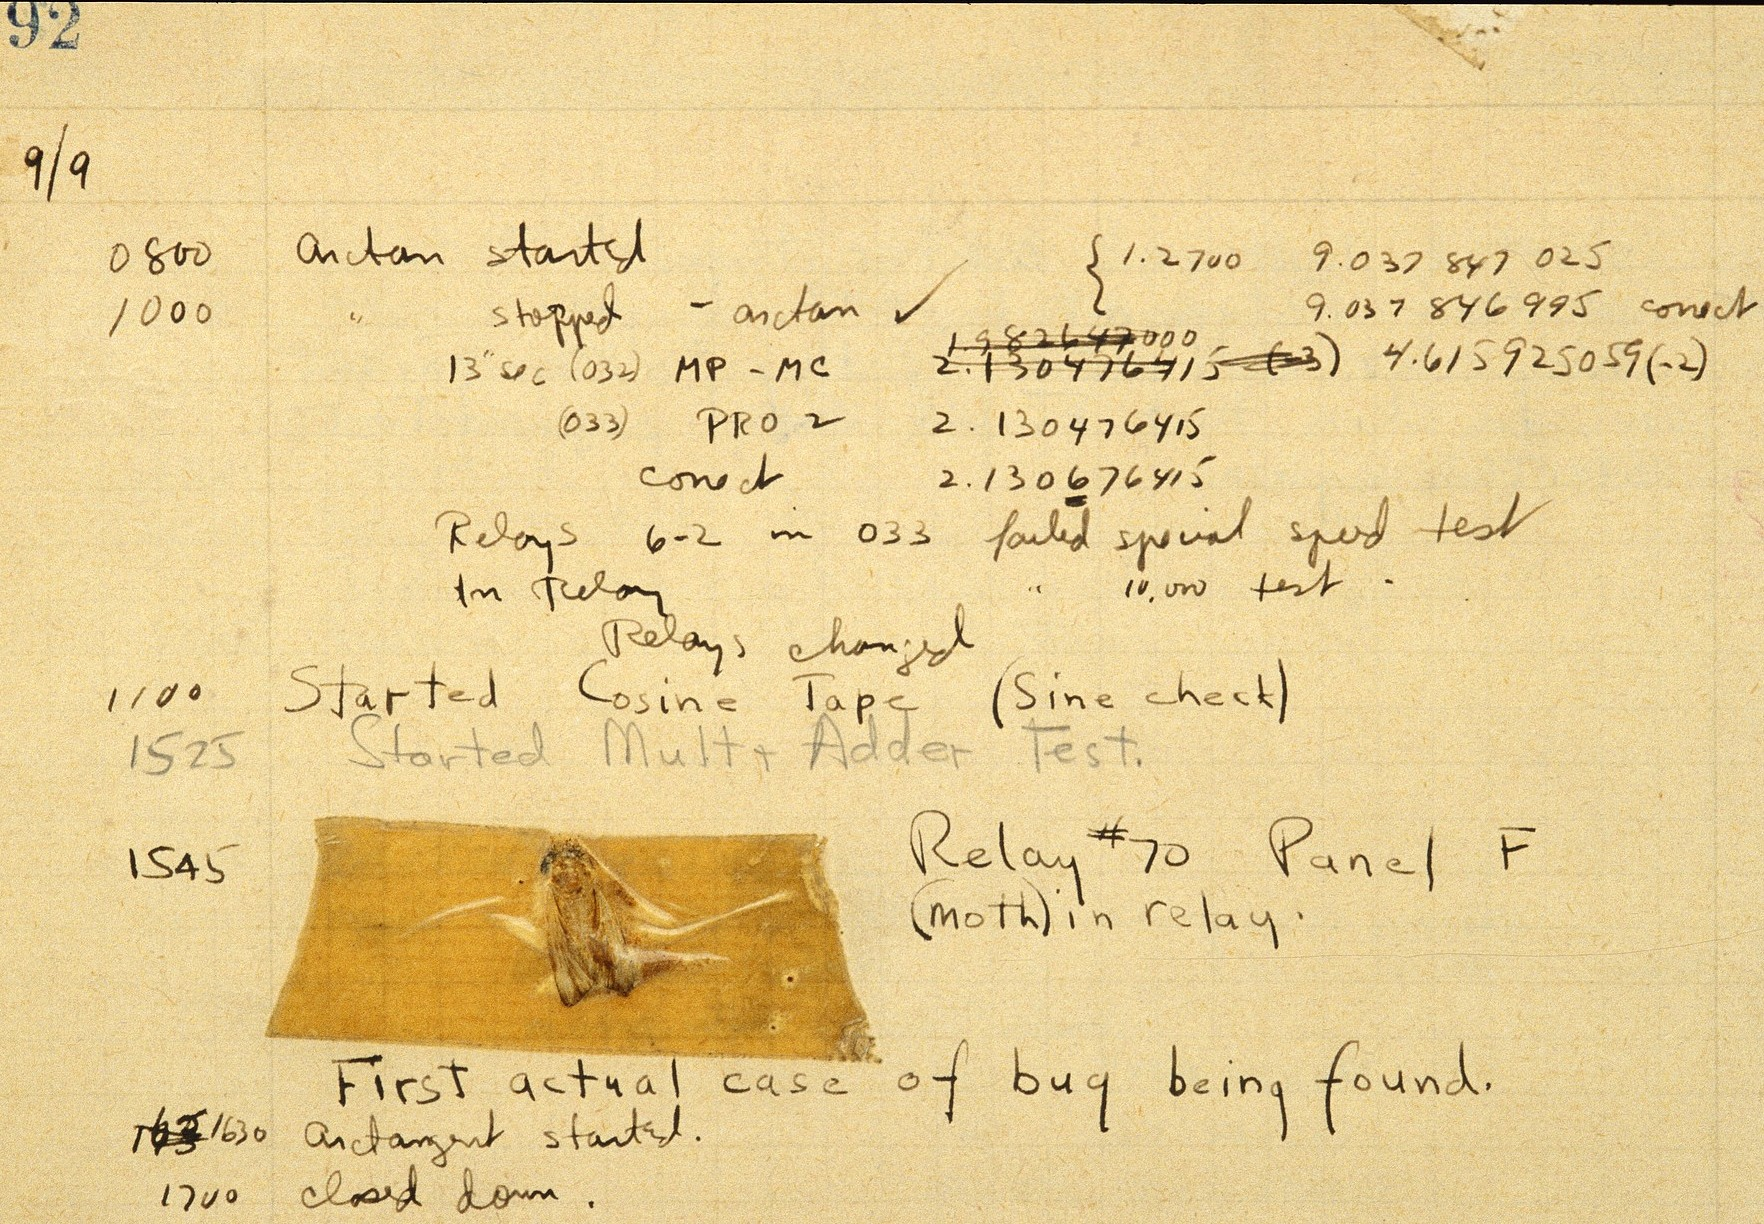
\includegraphics[width=0.9\textwidth]{c6.sub.bug.jpg}
  \end{figure}
\end{frame}

\begin{frame}
  \frametitle{子程序和Bugs | bug | \alert{实例}}
  \begin{block}{Perl脚本中常见的bug}
    \begin{itemize}
      \item 括号没配对
      \item 没用分号结尾
      \item 索引计算错误
      \item 变量/函数等拼写错误
      \item 本该用减法却用成了加法
      \item 意欲测试(==)却使用了赋值(=)
      \item 程序设计存在逻辑缺陷
      \item ……
    \end{itemize}
  \end{block}
\end{frame}

\subsection{use warnings;和use strict;}
\begin{frame}[fragile]
  \frametitle{子程序和Bugs | \alert{use warnings;和use strict;}}
  \begin{block}{use warnings;}
\begin{lstlisting}
#!/usr/bin/perl -w
use warnings;
perl -w script.pl
\end{lstlisting}
开启Perl的警告功能,尝试寻找代码中潜在的问题(如:变量不止声明了一次),并给出警告。
  \end{block}
  \pause
  \begin{block}{use strict;}
\begin{lstlisting}
use strict;
\end{lstlisting}
\begin{itemize}
  \item 强制声明变量(找到未声明的变量)
  \item 找到拼写错误的变量
  \item ……
\end{itemize}
  \end{block}
\end{frame}

\subsection{使用注释和print语句}
\begin{frame}
  \frametitle{子程序和Bugs | \alert{注释和print}}
  \begin{block}{选择性注释}
    \begin{itemize}
      \item 通过不断的试验,发现当注释掉某部分代码时错误信息消失了,就知道是哪里出错了。 
      \item 适用于没有精确定位错误位置、但是知道大体范围时。
    \end{itemize}
  \end{block}
  \pause
  \begin{block}{添加print语句}
    \begin{itemize}
      \item 添加print语句,打印出变量的值。
      \item 适用于差不多已经知道是哪儿出问题时。
    \end{itemize}
  \end{block}
\end{frame}

\subsection{Perl调试器}
\begin{frame}[fragile]
  \frametitle{子程序和Bugs | Perl调试器 | 程序6.4 | 用途}
  \begin{itemize}
    \item 程序处理一条序列和两个碱基
    \item 如果能够在序列中找到这两个碱基的话,就把从这两个碱基到序列末尾的所有内容输出出来
    \item 可以以命令行参数的形式把这两个碱基传递给程序
    \item 如果不给参数,默认使用TA这两个碱基
  \end{itemize}
\end{frame}

\begin{frame}[fragile]
  \frametitle{子程序和Bugs | Perl调试器 | 程序6.4.1}
\begin{lstlisting}[firstnumber=1]
#!/usr/bin/perl
# Example 6-4   A program with a bug or two
#
# An optional argument, for where to start printing the sequence,
#  is a two-base subsequence.
#
# Print everything from the subsequence ( or TA if no subsequence
# is given as an argument) to the end of the DNA.
\end{lstlisting}
\end{frame}

\begin{frame}[fragile]
  \frametitle{子程序和Bugs | Perl调试器 | 程序6.4.2}
\begin{lstlisting}[firstnumber=10]
# declare and initialize variables
my $dna = 'CGACGTCTTCTAAGGCGA';
my @dna;
my $receivingcommittment;
my $previousbase = '';

my $subsequence = '';

if (@ARGV) {
    my $subsequence = $ARGV[0];
}
else {
    $subsequence = 'TA';
}
\end{lstlisting}
\end{frame}

\begin{frame}[fragile]
  \frametitle{子程序和Bugs | Perl调试器 | 程序6.4.3}
\begin{lstlisting}[firstnumber=25,basicstyle=\small\tt]
my $base1 = substr( $subsequence, 0, 1 );
my $base2 = substr( $subsequence, 1, 1 );

# explode DNA
@dna = split( '', $dna );

######### Pseudocode of the following loop:
#
# If you've received a committment, print the base and continue.  Otherwise:
#
# If the previous base was $base1, and this base is $base2, print them.
#   You have now received a committment to print the rest of the string.
#
# At each loop, save the previous base.
\end{lstlisting}
\end{frame}

\begin{frame}[fragile]
  \frametitle{子程序和Bugs | Perl调试器 | 程序6.4.4}
\begin{lstlisting}[firstnumber=40,basicstyle=\small\tt]
foreach (@dna) {
    if ($receivingcommittment) {
        print;
        next;
    }
    elsif ( $previousbase eq $base1 ) {
        if (/$base2/) {
            print $base1, $base2;
            $recievingcommitment = 1;
        }
    }
    $previousbase = $_;
}

print "\n";

exit;
\end{lstlisting}
\end{frame}

\begin{frame}[fragile]
  \frametitle{子程序和Bugs | Perl调试器 | 程序6.4 | 输出}
  \begin{block}{实际输出}
\begin{lstlisting}[language=sh]
$ perl example 6-4 AA

$ perl example 6-4
TA
\end{lstlisting}
  \end{block}
  \pause
  \begin{block}{理论输出}
\begin{lstlisting}[language=sh]
$ perl example 6-4 AA
AAGGCGA
$ perl example 6-4
TAAGGCGA
\end{lstlisting}
  \end{block}
\end{frame}

\begin{frame}[fragile]
  \frametitle{子程序和Bugs | Perl调试器 | \alert{启动和停止}}
  \begin{block}{启动}
\begin{lstlisting}
# 交互式运行
perl -d script.pl

#自动启动
#!/usr/bin/perl -d
\end{lstlisting}
  \end{block}
  \pause
  \begin{block}{停止}
    在调试器中输入q即可。
  \end{block}
\end{frame}

\begin{frame}
  \frametitle{子程序和Bugs | Perl调试器 | \alert{常用命令}}
  %\begin{block}{常用命令}
  \begin{description}
    \item[man perldebug] Perl调试器的联机帮助页
    \item[h] 简短的帮助信息
    \item[h CMD] 特定命令的帮助信息
    \item[h h] 全部的帮助信息页
    \item[p] print,打印出表达式/变量的值
    \item[n] next,执行语句(把子程序看做单独的语句,直接跳过)
    \item[s] single,执行语句(进入子程序,一步一步运行)
    \item[v] view,查看临近的代码行
    \item[b] breakpoint,(在指定行)设置断点
    \item[c] continue,继续执行直到某个位置(比如:行,断点)
    \item[B] 删除(某行的)一个断点或者所有断点(B *)
    \item[w] watch,设置一个要查看/监视的表达式
    \item[R] restart,尝试重新运行程序
  \end{description}
  %\end{block}
\end{frame}

\begin{frame}[fragile]
  \frametitle{子程序和Bugs | Perl调试器 | \alert{补充说明}}
  \begin{itemize}
    \item 调试器显示的是将要执行的那一行代码,而不是已经执行的代码行
    \item 使用v查看临近代码行时,当前行(即将被执行的行)会以 \verb|==>|进行标明
    \item 重复键入v可以持续显示更多代码,使用减号 \verb|-| 会上翻一屏
    \item 使用print打印数组时(\verb|print @array|)默认元素之间没有空格,把数组放在双引号中(\verb|print "@array"|)会使元素以空格分隔的形式展示出来
    \item 所谓断点(breakpoint)指的是程序中的一个点,调试器会在此处停止执行(避免从头开始一步一步执行代码中的每一行),便于检查附近的代码
    \item 特殊变量 \verb|$_|:print和模式匹配等默认使用的变量
    \item 特殊变量 \verb|@_|:子程序存储参数的变量
    \item \verb|use warings;|和 \verb|use strict;|不是万能的,但强烈推荐同时使用它们两个
    \item 错误信息可能会有(一行)错位,所以真正的错误可能出现在提示行的前面
  \end{itemize}
\end{frame}

\section{回顾和总结}
\subsection{总结}
\begin{frame}
  \frametitle{子程序和Bugs | 总结}
  \begin{block}{知识点}
    \begin{itemize}
      \item 子程序:定义,调用,返回值,参数,作用域
      \item 命令行参数:特殊变量,提示信息,提取数组元素
      \item 传递数据给子程序:通过值,通过引用(引用与解引用)
      \item 模块:编写,使用,指定库目录
      \item 调试:use warnings;和use strict;,注释和print语句,调试器
      \item Perl调试器:启动和停止,常用命令,设置断点
    \end{itemize}
  \end{block}
  \pause
  \begin{block}{技能}
    \begin{itemize}
      \item 能够熟练使用子程序
      \item 能够调试Perl程序
      \item 能够熟练使用Perl调试器
    \end{itemize}
  \end{block}
\end{frame}

\subsection{思考题}
\begin{frame}
  \frametitle{子程序和Bugs | 思考题}
  \begin{enumerate}
    \item 如何定义和调用子程序?
    \item 举例说明作用域的概念。
    \item 如何获取命名行参数?
    \item 给子程序传递数据的方法有哪些?举例说明。
    \item 总结调试Perl程序的方法。
    \item 如何使用Perl调试器对程序进行调试?
  \end{enumerate}
\end{frame}

\begin{frame}
  \frametitle{下节预告}
  回顾在Linux中有哪些方法可以实现随机化,或者随机选取一行/多行?\\
  (提示:sort,shuf)
\end{frame}


\section*{Acknowledgements}
\begin{frame}
  \frametitle{Powered by}
  \begin{center}
    
\includegraphics[width=9cm]{power.png}
  \end{center}
\end{frame}

\end{document}

